\documentclass{beamer}
\usepackage[utf8]{inputenc}

\usetheme{Madrid}
\usecolortheme{default}
\usepackage{amsmath,amssymb,amsfonts,amsthm}
\usepackage{txfonts}
\usepackage{tkz-euclide}
\usepackage{listings}
\usepackage{adjustbox}
\usepackage{array}
\usepackage{tabularx}
\usepackage{gvv}
\usepackage{lmodern}
\usepackage{circuitikz}
\usepackage{tikz}
\usepackage{graphicx}
\usepackage{multicol}

\setbeamertemplate{page number in head/foot}[totalframenumber]

\usepackage{tcolorbox}
\tcbuselibrary{minted,breakable,xparse,skins}



\definecolor{bg}{gray}{0.95}
\DeclareTCBListing{mintedbox}{O{}m!O{}}{%
  breakable=true,
  listing engine=minted,
  listing only,
  minted language=#2,
  minted style=default,
  minted options={%
    linenos,
    gobble=0,
    breaklines=true,
    breakafter=,,
    fontsize=\small,
    numbersep=8pt,
    #1},
  boxsep=0pt,
  left skip=0pt,
  right skip=0pt,
  left=25pt,
  right=0pt,
  top=3pt,
  bottom=3pt,
  arc=5pt,
  leftrule=0pt,
  rightrule=0pt,
  bottomrule=2pt,
  toprule=2pt,
  colback=bg,
  colframe=orange!70,
  enhanced,
  overlay={%
    \begin{tcbclipinterior}
    \fill[orange!20!white] (frame.south west) rectangle ([xshift=20pt]frame.north west);
    \end{tcbclipinterior}},
  #3,
}
\lstset{
    language=C,
    basicstyle=\ttfamily\small,
    keywordstyle=\color{blue},
    stringstyle=\color{orange},
    commentstyle=\color{green!60!black},
    numbers=left,
    numberstyle=\tiny\color{gray},
    breaklines=true,
    showstringspaces=false,
}
%------------------------------------------------------------
%This block of code defines the information to appear in the
%Title page
\title %optional
{2.10.58}
\date{September 6,2025}


\author 
{Jnanesh Sathisha karmar - EE25BTECH11029}



\begin{document}



\frame{\titlepage}
\begin{frame}{Question}
 Let $\vec{P},\vec{Q},\vec{R}\  \text{and}\  \vec{S}$ be the points on the plane with position vectors $-2\hat{i} -\hat{j}, 4\hat{i}, 3\hat{i} + 3\hat{j}$
and $-3\hat{i} + 2\hat{j}$ respectively. The quadrilateral $\vec{PQRS}$ must be a
\begin{enumerate}
\begin{multicols}{1}
    \item parallelogram, which is neither a rhombus nor a rectangle
    \item square
    \item rectangle, but not a square
    \item rhombus, but not a square
\end{multicols}
\end{enumerate}
\end{frame}



\begin{frame}{Equation}
Given details:
\begin{align}
    \vec{P}=\myvec{-2\\-1\\0}\ \vec{Q}=\myvec{4\\0\\0}\ 
    \vec{R}=\myvec{3\\3\\0}\ 
    \vec{S}=\myvec{-3\\2\\0}
\end{align}
\end{frame}
\begin{frame}{Theoretical Solution}

Finding the sides:
\begin{align}
\vec{Q}-\vec{P}=\myvec{6\\1\\0} \  \vec{R}-\vec{Q}=\myvec{-1\\3\\0} \\
\vec{S}-\vec{R}=\myvec{-6\\-1\\0} \ 
\vec{P}-\vec{S}=\myvec{1\\-3\\0}
\end{align}
\end{frame}

\begin{frame}{Theoretical Solution}
First let's check wheter the given opposite sides of the quadrilateral are parallel to each other \\
For the sides to be parallel 
\begin{align}
    \vec{Q-P}=\vec{S-R}\\
    \vec{R-Q}=\vec{P-S}\\
\end{align}
Since:
\begin{align}
    \vec{Q-P}=\vec{R-S}=\myvec{6\\1\\0}\\
    \vec{R-Q}=\vec{S-P}=\myvec{-1\\3\\0}
\end{align}

\end{frame}


\begin{frame}{Theoretical Solution}
Therefore the opposite sides are parallel to each other and Thus the given quadrilateral can be classified as a \textbf{Parallelogram}.\\Now, checking for right angle, we check for inner product.
\begin{align}
 \brak{\vec{Q}- \vec{P}}^{\top} \brak{\vec{R}- \vec{Q}}=\myvec{6 & 1&0}\myvec{-1 \\3\\0}=-3
\end{align}
This implies that the parallelogram is neither a rectangle nor a square \\

\end{frame}
\begin{frame}{Theoretical Solution}
Checking for a rhombus:\\
The given quadrilateral is a rhombus if its diagonals are orthogonal,
\begin{align}
\brak{\vec{R}- \vec{P}}^{\top} \brak{\vec{S}- \vec{Q}}=\myvec{5 & 4&0}\myvec{-7\\ 2\\0}=-27
\end{align}
\end{frame}
\begin{frame}{Theoretical Solution}
We can see that $\brak{\vec{R}- \vec{P}}^{\top} \brak{\vec{S}- \vec{Q}}$ is not equal to $0$, that is, the diagonals are not orthogonal and therefore the quadrilateral $\vec{P}\vec{Q}\vec{R}\vec{S}$ is a parallelogram which is neither a rhombus nor a rectangle.\\
\end{frame}



\begin{frame}[fragile]
    \frametitle{C Code (1) - Function to store the points }

    \begin{lstlisting}

#include <stdio.h>

void get_points(double *points) {
    double coords[8] = {-2,-1,  4,0,  3,3,  -3,2};

    for (int i = 0; i < 8; i++) {
        points[i] = coords[i];
    

}
}



    \end{lstlisting}
\end{frame}


\begin{frame}[fragile]
    \frametitle{Python Code - Using Shared Object}
    \begin{lstlisting}

import ctypes
import numpy as np
import matplotlib.pyplot as plt

parallelogram_lib = ctypes.CDLL("./points.so")

parallelogram_lib.get_points.argtypes = [np.ctypeslib.ndpointer(dtype=np.double, ndim=1, flags="C")]

points = np.zeros(8, dtype=np.double)

parallelogram_lib.get_points(points)






\end{lstlisting}
\end{frame}

\begin{frame}[fragile]
    \frametitle{Python Code - Using Shared Object}
    \begin{lstlisting}
points = points.reshape((4,2))

points = np.vstack([points, points[0]])

plt.plot(points[:,0], points[:,1], "bo-")
plt.title("Paralleogram from C library")
plt.xlabel("X")
plt.ylabel("Y")
plt.gca().set_aspect("equal")
plt.grid(True)
plt.savefig('figs/parallelogram.png')
subprocess.run(shlex.split('termux-open ../figs/parallelogram.png'))
plt.show()


\end{lstlisting}
\end{frame}



\begin{frame}{Plot-Using Both C and Python}
    \centering
    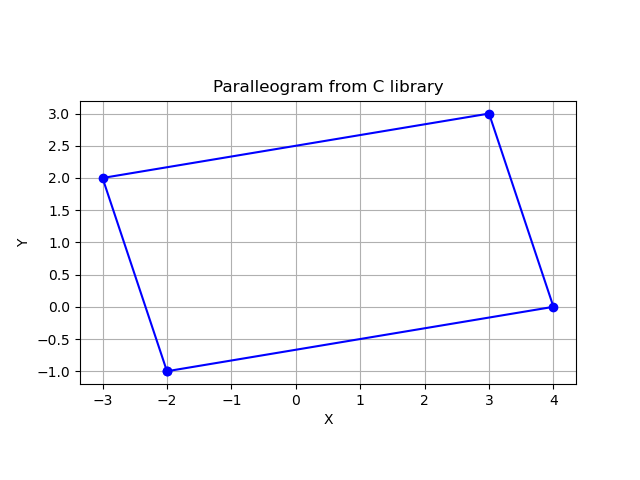
\includegraphics[width=\columnwidth, height=0.8\textheight, keepaspectratio]{figs/parallelogram.png}     
\end{frame}

\begin{frame}[fragile]
    \frametitle{Python Code}
    \begin{lstlisting}
import numpy as np
import matplotlib.pyplot as plt

points=np.array([[-2,-1],[4,0],[3,3],[-3,2]])
points=np.vstack([points,points[0]])
plt.plot(points[:,0],points[:,1],"bo-",linewidth=2)
plt.title("Parallelogram of 4 Points")
plt.xlabel("X-axis")
plt.ylabel("Y-axis")
plt.gca().set_aspect("equal")
plt.grid(True)
plt.savefig('figs/parallelogram2.png')
subprocess.run(shlex.split('termux-open ../figs/parallelogram.png'))
plt.show()









\end{lstlisting}
\end{frame}





\begin{frame}{Plot-Using only Python}
    \centering
    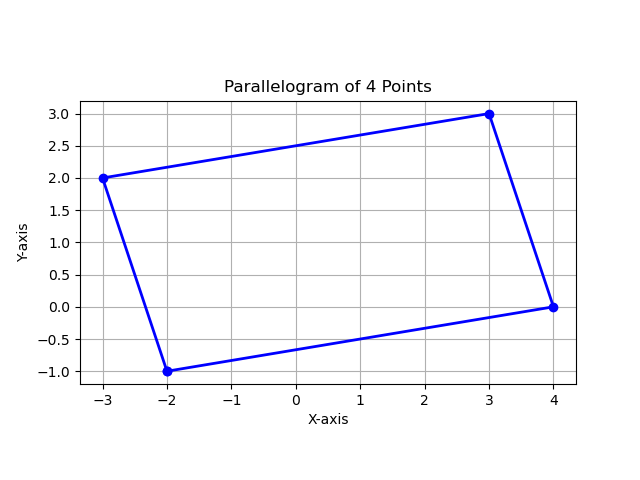
\includegraphics[width=\columnwidth, height=0.8\textheight, keepaspectratio]{figs/parallelogram2.png}     
\end{frame}


\end{document}